\section{Work left before submitting the thesis}
\label{sec:future_work}

The three articles written as first author presented in~\autoref{sec:submitted} will consist the majority of the thesis by articles.
Additionally, to maximize the value of the data gathered, especially through the work related to~\ac{DRIVE}, a few additional experiments will be conducted.
First, an analysis of the performance improvement that can be reached through dynamic modelling for navigation on ice will be conducted.
Second, an investigation of the limit of current adaptive models will be conducted by artificially mixing datasets on different terrains.
Thirdly, we will study of the impact of~\ac{DRIVE}~\ac{UGV} characterization on path following performance under a realistic deployment setting.
These results will be appended to the published and submitted articles in the thesis to complete it.
A schedule for the remaining work and Gantt chart are presented in~\autoref{sec:schedule}

\subsection{Dynamic modeling on ice}
We learned through our~\ac{DRIVE} work that slip learning model reach their functional limit under extreme conditions, such as navigation on an ice rink, as shown in~\autoref{fig:warthog-ice}.
Indeed, the low wheel-to-ground friction leads to high motion inertia, which is not modeled by slip learning.
While a lot of attention is given to generate and validate dynamic motion model for high-speed driving on concrete~\citep{Djeumou2023} or gravel~\citep{Williams2018}, not much work has focused on investigating their functionality on ice.
Since we have already completed the work to collect a~\SI{20}{\min} dataset of uniform vehicle input sampling, the time required to investigate the predictive performance of dynamic models on this dataset is much smaller.
\begin{SCfigure}[\sidecaptionrelwidth][h!]
	\centering
	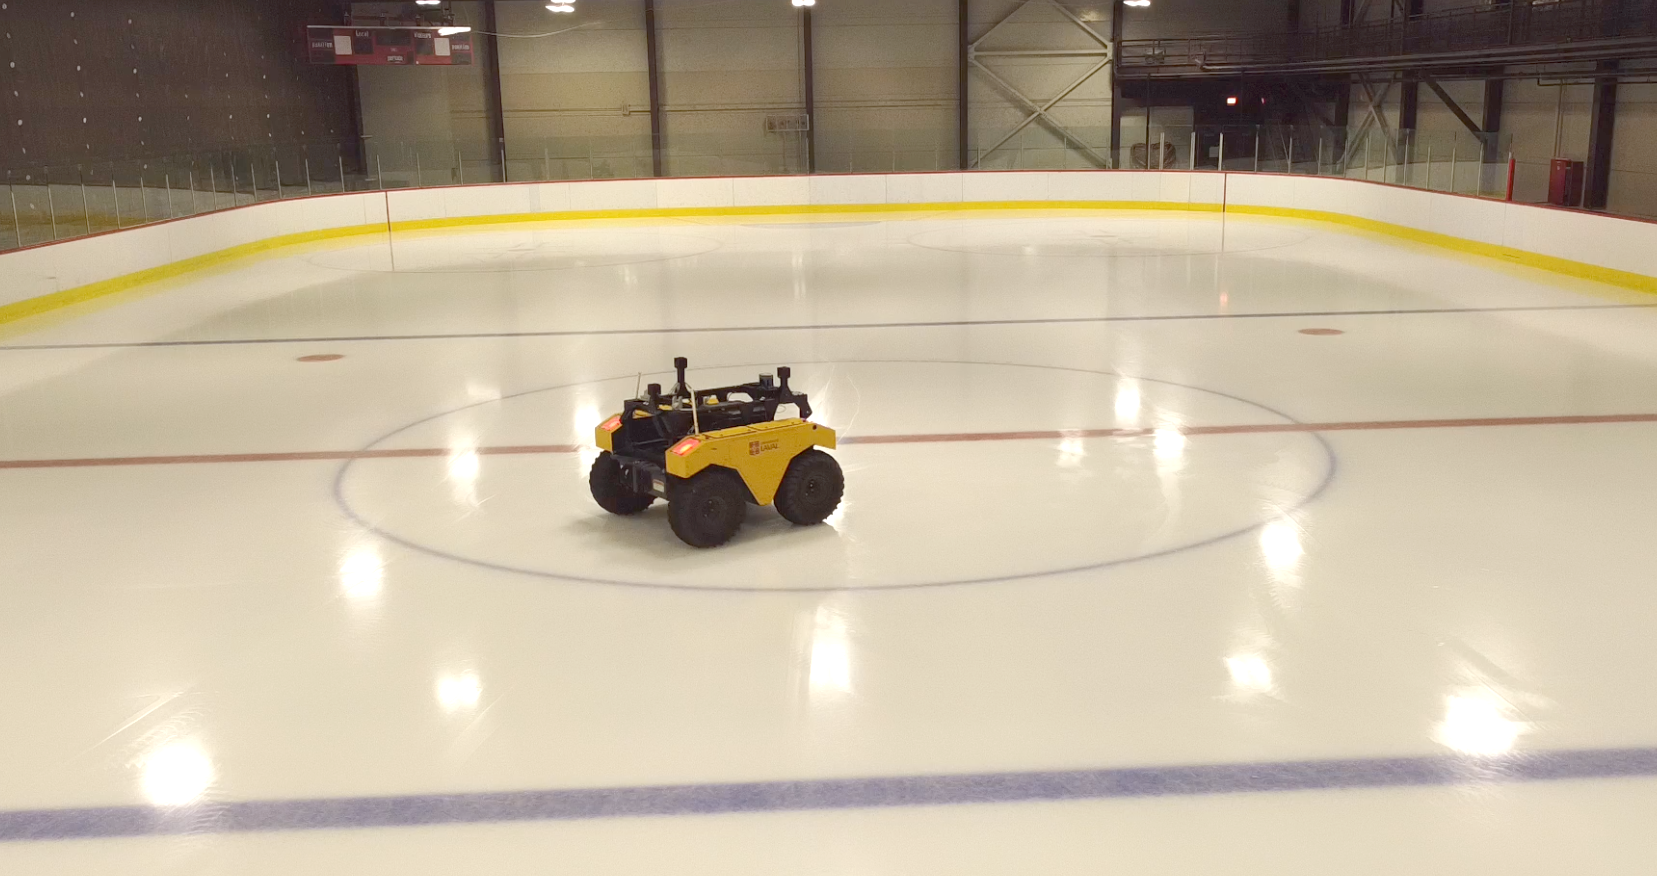
\includegraphics[width=0.7\textwidth]{figs/warthog_ice.png}
	\caption{
		A photo is the Warthog, our~\SI{470}{\kilo\gram} research~\ac{SSMR}.
		Via the~\ac{DRIVE} protocol, we have collected a~\SI{20}{\min} dataset of the vehicle exectuting a large spectrum of commands.
		This dataset shows the limit of our current slip learning model, motivating an investigation of dynamic model performance.
	}
	\label{fig:warthog-ice}
\end{SCfigure}

This work could lead to contributions related to dynamic formulation for~\acp{SSMR} navigating on ice, or learning dynamic model parameters through~\ac{BLR} to facilitate deployment of dynamic models.
The evaluation pipeline for model training and prediction error over an entire dataset is already set up and ready to compare dynamic models to slip learning.\footnote{\url{https://github.com/norlab-ulaval/norlab_WMRD}}
Improvements could also be made to the~\ac{DRIVE} protocol to sample additional dynamic variables, such as body acceleration.
\subsection{Adaptive motion modeling}
Next, I plan to study the performance of adaptive modeling under extreme traction variation.
To illustrate this challenge, \autoref{fig:snow_var} shows two use cases, namely hard and deep snow navigation, for which traction varies significantly.
In the case of deep snow navigation, the~\ac{SSMR} almost reached immobilization, which means that switching between both conditions produces the almost the largest change in traction conditions that can be observed for a specific~\ac{UGV}.
This is an ideal case to investigate the limits of current adaptive modeling approach, which are easy to integrate with our slip learning model.
\begin{figure}[h!]
	\begin{center}
		\begin{subfigure}[b]{0.49\textwidth}
			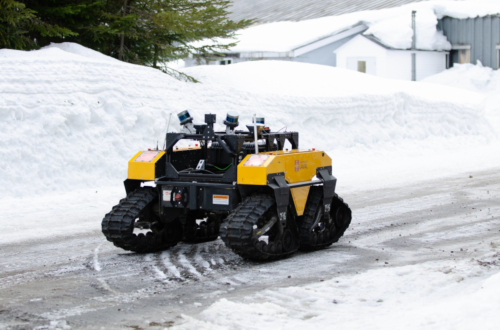
\includegraphics[width=\linewidth]{figs/warthog_hard_snow.pdf}
			\caption{}
			\label{fig:hard_snow}
		\end{subfigure}%
		~
		\begin{subfigure}[b]{0.49\textwidth}
			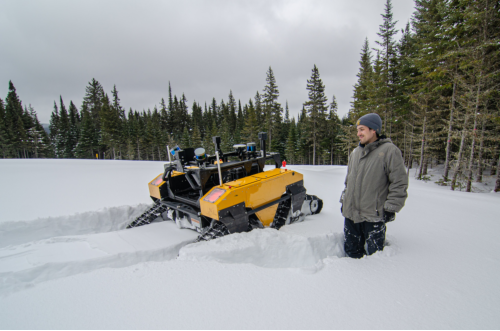
\includegraphics[width=\linewidth]{figs/snow_depth.pdf}
			\caption{}
			\label{fig:deep_snow}
		\end{subfigure}%
		\caption{
		Example of distinct terrain navigating encountered during wintertime off-road navigation with the Warthog platform.
		\textbf{(a)}: Hard snow navigation, with limited slip, representing nominal navigation.
		\textbf{(b)}: Deep snow navigation, with high slip, representing an edge case for~\ac{SSMR} motion modeling.
		}
		\label{fig:snow_var}
	\end{center}
\end{figure}

As proposed by~\citet{Mckinnon2019}, weighted~\ac{BLR} learning enables re-training of the model based on new traction conditions and a prior motion model.
In their work, they show that weighted~\ac{BLR} performs well to adapt to slight changes in traction condition, both artificially generated and through slope variation.
However, no study investigates the performance of adaptive modeling with respect to the degree of traction variability and what is the operational limit.
By leveraging the~\ac{DRIVE} protocol to gather two distinct datasets, namely on hard and deep snow, we could simulate such changes in traction and analyse the performance of weighted~\ac{BLR} learning.
In the case of failure, it will be an opportunity to develop improvements to this adaptive modeling approach, increasing its robustness to significant variation in traction.

\subsection{\ac{DRIVE} impact on path following}
Lastly, we have developed a predictive control library in the context of industrial demonstrations for this project.\footnote{\url{https://github.com/norlab-ulaval/norlab_controllers}}
Such controllers are based on the~\ac{MPC} algorithm, enabling high speed path following with low tracking error.
In our case, we have implemented a simplified version of the slip-aware~\ac{MPC} controlled proposed by~\citet{Hewing2020}.
Since the motion model acts as a interchangeable module for such controllers, the prediction accuracy improvements reached through our work on the~\ac{DRIVE} protocol will most likely improve~\ac{MPC} path following performance.
A last interesting result would be to quantify the path following error improvement reached through training the slip learning model with a~\ac{DRIVE}-gathered training dataset instead of manual driving.
Typically, human driving data is limited in driving velocity since it is the first time for which the vehicle navigated the target trajectory.
Our hypothesis is that by training the model through~\ac{DRIVE}, path following performance at high speed is improved as soon as the first time the~\ac{UGV} executes the desired trajectory.

\subsection{Schedule for upcoming work}
\label{sec:schedule}

In this section, a plan for the upcoming steps for this thesis is presented. 
A Gantt chart is shown in~\autoref{fig:gantt}, providing visual support for the planning presented.
The remaining work is split into three main categories, namely thesis writing, \emph{ICRA} paper finalization and thesis review and defense.

The thesis will be written via articles insertion, where the articles selected are presented in~\autoref{sec:first_author}.
This task will require appending every article which will represent a distinct thesis chapter.
Mathematical notation will be modified to be uniform for all articles and facilitate thesis reading and review.
Then, I will write on writing the final chapter, which will present the results of the experiments describes in~\autoref{sec:future_work}.
My planning is to invest half days on thesis writing and the other half days on final experiments to maintain motivation through the writing process.
For these final experiments, I will focus on dynamic modeling during the first two months since the data is already recorded and the result can be produced generally faster.
Then, when winter comes, I will record the data for the hard and deep snow experiments and produce the results in the first two months of 2024.
Final chapter writing will be done simultaneously as those last experiments are conducted.

Furthermore, since our work on~\ac{DRIVE} is undergoing the peer review process, we will receive the results in January 2024.
Paper improvements will need to be prioritized at this time for paper re-submission which will most likely be due for end of January 2024.
Then, the official paper presentation will be done during the three weeks leading to the conference, including a dry run in the laboratory to fetch initial feedback and maximize the presentation quality.
Then, from May 14th to 17th 2024, I will attend the conference to present our paper on site.
In the case the paper is rejected at the conference, the reviews will still be into account and the paper will be improved and re-submitted to an alternative venue.
In this case, slight changes to the planning presented in this section will be made to ensure thesis defense still happens in August 2024.

Lastly, once the thesis is submitted, a delay will originate
%TODO: Complete this section with ULAVAL standards.

\setlength{\fboxsep}{9pt}
\begin{figure}[htbp]
	\centering
	\definecolor{navyblue}{RGB}{21,80,130}
\setganttlinklabel{f-s}{}

\begin{ganttchart}[
     %Specs 0.43 0.43 1
     y unit title=0.43cm,
     y unit chart=0.55cm,
     x unit=1.1cm,  %1.2cm
     vgrid={*{1}{draw=none},*{1}{black}},
     title height=1,   %1
     title label font=\bfseries\footnotesize,
     % bar 0.4 10pts
     bar/.style={fill=navyblue},
     bar height=0.4,
     bar label font=\footnotesize,
     bar label node/.append style={left=10pt},  %10
     % group 0 0.6 0.3 0.2 0.3 10pts
     group right shift=0,
     group top shift=0.6,
     group height=.3,
     group peaks width={0.2},
     group peaks height={0.3},
     group label node/.append style={left=10pt},
     group label font=\bfseries\footnotesize,
     % milestone 0.4 1 10pts
     milestone/.append style={xscale=0.4, yscale=1},
     milestone label node/.append style={left=10pt},
     milestone label font=\itshape\footnotesize
     ]{1}{8}
    \gantttitle[]{2024}{8}
    \\              
    \gantttitle{J}{1} \gantttitle{F}{1} \gantttitle{M}{1} 
    \gantttitle{A}{1} \gantttitle{M}{1} \gantttitle{J}{1} 
    \gantttitle{J}{1} \gantttitle{A}{1} 
    \\
    %--------------------------------------       
    \ganttgroup{Thesis writing}{1}{3}\\
    
    \ganttbar{Articles insertion}{1}{1}
    \ganttbar[inline, bar label font/.append=\color{white}]{}{1}{1}\\
    
    \ganttbar{Final results chapter}{2}{2}
    \ganttbar[inline, bar label font/.append=\color{white}]{}{2}{2}\\
    
    \ganttbar{Introduction, conclusion}{3}{3}
    \ganttbar[inline, bar label font/.append=\color{white}]{}{3}{3}\\
	
	\ganttmilestone{Thesis submitted}{3}\\
	
    %--------------------------------------       
    \ganttgroup{Final experiments}{1}{2} \\ 
    
    \ganttbar{DRIVE impact on UGV path following}{1}{2}
    \ganttbar[inline, bar label font/.append=\color{white}]{}{1}{2}\\
    
    %--------------------------------------       
    \ganttgroup{\emph{ICRA 2024}}{2}{5} \\ 
    
    \ganttbar{Paper corrections}{2}{2}
    \ganttbar[inline, bar label font/.append=\color{white}]{}{2}{2}\\
    
    \ganttmilestone{Re-submission}{2}\\
    
    \ganttbar{Presentation preparation}{5}{5}
    \ganttbar[inline, bar label font/.append=\color{white}]{}{5}{5}\\
    
    \ganttmilestone{Article presentation}{5}\\
    
    %--------------------------------------       
    \ganttgroup{Thesis defense}{4}{8}\\
    
    \ganttbar{Thesis review}{4}{6}
    \ganttbar[inline, bar label font/.append=\color{white}]{}{4}{6}\\
    
    \ganttbar{Defense preparation}{4}{6}
    \ganttbar[inline, bar label font/.append=\color{white}]{}{4}{6}\\
    
    \ganttmilestone{Defense}{6}\\
    
    \ganttbar{Final reviews}{7}{8}
    \ganttbar[inline, bar label font/.append=\color{white}]{}{7}{8}\\
    
    \ganttmilestone{Final submission}{8}\\
    
\end{ganttchart}

	\caption{Gantt chart of the remaining tasks left to do to complete this thesis and planning for their completion leading to August 2024.}
	\label{fig:gantt}
\end{figure}
\setlength{\fboxsep}{12pt}
